\documentclass[a4paper,11pt]{article}
\input{/home/tof/Documents/Cozy/latex-include/preambule_doc.tex}
\input{/home/tof/Documents/Cozy/latex-include/preambule_commun.tex}
\newcommand{\showprof}{show them}  % comment this line if you don't want to see todo environment
\setlength{\fboxrule}{0.8pt}
\fancyhead[L]{\fbox{\Large{\textbf{Tris 01}}}}
\fancyhead[C]{\textbf{Trier des cartes}}
\newdate{madate}{10}{09}{2020}
%\fancyhead[R]{\displaydate{madate}} %\today
%\fancyhead[R]{Seconde - SNT}
\fancyhead[R]{Première - NSI}
%\fancyhead[R]{Terminale - NSI}
\fancyfoot[L]{\vspace{1mm}Christophe Viroulaud}
\AtEndDocument{\label{lastpage}}
\fancyfoot[C]{\textbf{Page \thepage/\pageref{lastpage}}}
\fancyfoot[R]{\includegraphics[width=2cm,align=t]{/home/tof/Documents/Cozy/latex-include/cc.png}}

%DODO commencer par algo recherche mini (voir https://www.youtube.com/watch?v=AgtOCNCejQ8 vers 2min)
\begin{document}
\section{Problématique}
Trier un jeu de cartes est une opération qui peut paraître triviale, mais qui ouvre des enjeux essentiels dans le contexte des données. En effet, on demande régulièrement à une machine de manipuler et donc trier des quantités importantes d'informations et il convient alors d'élaborer des algorithmes rigoureux.
\begin{center}
    \framebox{Existe-t-il plusieurs méthodes pour trier des données?}
\end{center}
\section{Trier des cartes manuellement}
\begin{center}
\centering
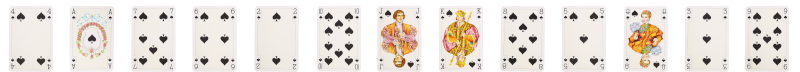
\includegraphics[width=17cm]{ressources/cartes-pique.png}
\captionof{figure}{Cartes mélangées}
\label{pique}
\end{center}
\begin{activite}
\begin{enumerate}
    \item Prendre le paquet de cartes mélangées et les étaler sur la table.
    \item Trier les cartes.
    \item Formaliser la méthode utilisée sous forme d'un algorithme.
\end{enumerate}
\end{activite}
On distingue deux algorithmes:
\begin{center}
\begin{lstlisting}[language=bash]
Pour chaque carte du tas
    Trouver la plus petite carte dans la partie non triée.
    Échanger cette carte avec la première de la partie non triée.
\end{lstlisting}
\captionof{code}{Tri par sélection (en place)}
\label{CODE}
\end{center}
\begin{center}
    \begin{lstlisting}[language=bash]
Pour chaque carte du tas
    Mémoriser la carte en cours
    Décaler vers la droite toutes les cartes précédentes, supérieures à la carte en cours.
    Insérer la carte en cours dans l'espace vide.
    \end{lstlisting}
    \captionof{code}{Tri par insertion (en place)}
    \label{CODE}
    \end{center}
\section{Transposer au tri de données}
%effet de bord: variable mutable; présenter fonction sort()
\subsection{Tri par sélection}
\subsubsection{Implémentation}
\begin{activite}
\begin{enumerate}
    \item Écrire la fonction \textbf{trouver\_mini(tab: list) $\rightarrow$ int} qui renvoie l'indice du plus petit élément de \emph{tab}.
    \item Adapter la fonction précédente pour renvoyer l'indice du plus petit élément de \emph{tab}, compris entre l'indice \emph{i\_depart} et la fin du tableau. La signature de la fonction deviendra \textbf{trouver\_mini(tab: list, i\_depart: int) $\rightarrow$ int}.
    \item Écrire la fonction \textbf{echanger(tab: list, i: int, j: int) $\rightarrow$ None} qui échange les éléments d'indice \emph{i} et \emph{j} du tableau \emph{tab}.
    \item Écrire la fonction \textbf{tri\_selection(tab: list) $\rightarrow$ None} qui effectue un tri par sélection sur \emph{tab}.
    \item Construire par compréhension un tableau des entiers de 1 à 13.
    \item Mélanger le tableau à l'aide de la méthode \emph{shuffle} de la bibliothèque \emph{random}.
    \item Trier le tableau à l'aide de la fonction \emph{tri\_selection}.
\end{enumerate}
\end{activite}
\subsubsection{Terminaison}
La terminaison de la fonction est triviale. Le tri est composé de deux boucles bornées donc qui terminent.
\subsubsection{Correction}
Avant chaque itération de la boucle externe, la partie gauche du tableau est triée.
\subsubsection{Complexité}
Il convient de se demander si cette méthode de tri est efficace. Remarquons que le nombre d'opérations effectuées dépend du nombre \emph{n} d'éléments dans le tableau:
\begin{itemize}
    \item à la première itération de \emph{i}, la boucle de la fonction \emph{trouver\_mini} effectue \emph{n-1} itérations.
    \item à la deuxième itération de \emph{i}, la boucle de la fonction \emph{trouver\_mini} effectue \emph{n-2} itérations.
    \item \dots
\end{itemize}
\begin{aretenir}[]
Le tri par sélection effectue $\dfrac{n.(n-1)}{2}$ opérations pour ordonner le tableau. Le nombre d'opérations dépend de $n^2$.
\end{aretenir}
\subsection{Tri par insertion}
\subsubsection{Implémentation}
\begin{activite}
\begin{enumerate}
    \item Écrire la fonction \textbf{tri\_insertion(tab: list) $\rightarrow$None} en s'appuyant sur l'algorithme. Les indications suivantes permettront de construire les trois étapes:
    \begin{itemize}
        \item \underline{Mémoriser:} définir une variable \emph{en\_cours}, élément en cours de placement et \emph{pos}, position actuelle de cet élément.
        \item \underline{Décaler:} utiliser une boucle non bornée pour décaler les éléments vers la droite.
        \item \underline{Insérer:} placer l'élément \emph{en\_cours} à la nouvelle position \emph{pos}.
    \end{itemize}
    \item Tester la fonction sur un tableau.
\end{enumerate}
\end{activite}
\subsubsection{Terminaison}
Il faut se focaliser sur la boucle interne, non bornée.
\begin{activite}
Déterminer un variant de la boucle, qui prouve la terminaison.
\end{activite}
\subsubsection{Correction}
Comme pour le tri sélection, avant chaque itération de la boucle externe, la partie gauche du tableau est triée.
\subsubsection{Complexité}
La boucle externe effectue \emph{n} itérations dans tous les cas. Cependant, le nombre d'itérations de la boucle interne peut varier.
\begin{activite}
\begin{enumerate}
    \item Compter le nombre d'itérations de la boucle interne si le tableau est déjà trié.
    \item Compter le nombre d'itérations de la boucle interne si le tableau est trié dans l'ordre décroissant.
\end{enumerate}
\end{activite}
\begin{aretenir}[]
Le tri par insertion effectue un nombre moyen d'opérations qui dépend de $n^2$.
\end{aretenir}
\end{document}